% vim: tw=80 cc=81 spelllang=cs spell

\documentclass[11pt, a4paper, oneside, openany, draft]{book}

% Input and output encoding
\usepackage[utf8]{inputenc}
\usepackage[T1]{fontenc}

\usepackage[czech]{babel}

\usepackage[usenames,dvipsnames]{xcolor}
\usepackage{lmodern}
\usepackage{enumitem}
\usepackage{todonotes}
\usepackage{setspace}
\usepackage{graphicx}
\usepackage{amssymb,amsmath}
\usepackage{mathtools}
\usepackage{float}
\usepackage[pass]{geometry}
\usepackage{ifdraft}

% Theorems – add your own environments, should you need them.
\usepackage{amsthm}
\newtheorem{theorem}{Věta}

% Source code listings
\usepackage[draft=false]{minted}
\usemintedstyle{friendly}
\newminted{hs}{autogobble,linenos}

% Algorithms
\usepackage[Algoritmus]{algorithm}

\usepackage[ unicode=true,
             plainpages=false,
             pdfpagelabels,
             draft=false,
             hyperfootnotes=false,
             linkcolor={Sepia},
             citecolor={PineGreen},
             urlcolor={MidnightBlue},
           ]{hyperref}

\hypersetup{
    pdfauthor={Tvoje máma},
    pdftitle={Tohle je zasraná šablona na diplomku},
    pdfsubject={Bakalářská práce}
}

\usepackage[backend=bibtex8,
            bibencoding=UTF8
            maxnames=100
           ]{biblatex}
\addbibresource{bibliography.bib}

\setlength{\tabcolsep}{6pt}

% Macros for linking sections suitable for use in Czech text.
% e.g., v \myref{somelabel}{sekci} → v sekci 5.2
%       v \ymref{somelabel}{kapitole} → v 5. kapitole
\newcommand{\myref}[2]{\hyperref[#2]{#1~\ref*{#2}}}
\newcommand{\ymref}[2]{\hyperref[#1]{\ref*{#1}.~#2}}

% % % % % % % % % % % % % % % % % % % % % % % % % % % % % % % % % % % % % % % % 

\begin{document}
\frontmatter
\pagestyle{empty}

\begin{center}
{\Large \textsc{Masarykova univerzita}}

{\large \textsc{fakulta informatiky}}
    \vskip4em
    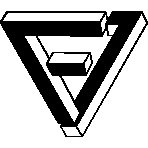
\includegraphics[width=4cm, height=4cm, draft=false] {logo_fi}
    \vskip4em
        {\begin{spacing}{1}
             \Huge \textbf{Musikk. A music streaming platform with social features.} % XXX: Title
    \end{spacing}}
    \vskip2em
        {\Large \textsc{Bachelor's Thesis}} % XXX: Type
    \vskip2em
        {\LARGE \textbf{Kirill Vorozhtsov}} % XXX: Author
    \vfill
    {\hfill\large Brno, 2025} % XXX: Year
\end{center}

\cleardoublepage
\restoregeometry

\section*{Prohlášení} Prohlašuji, že tato práce je mým původním autorským dílem,
které jsem vypracoval samostatně. Všechny zdroje, prameny a literaturu, které
jsem při vypracování používal nebo z~nich čerpal, v~práci řádně cituji
s~uvedením úplného odkazu na příslušný zdroj.

\vfill\noindent
\textbf{Vedoucí práce:} Tvá babka   % XXX
\cleardoublepage

\section*{Poděkování} % XXX
\cleardoublepage

\section*{Shrnutí} % XXX

\subsection*{Klíčová slova} % XXX


\setcounter{tocdepth}{2}
\tableofcontents
\pagestyle{plain}

\mainmatter
% vim: spell spelllang=cs


\chapter{Introduction}

% vim: spell spelllang=cs
\chapter{Usage}

\appendix
\input{chapters/archive}

\backmatter
\chapter{Literatura}
\begingroup
\raggedright
\printbibliography[heading=none]
\endgroup

\ifoptiondraft{\listoftodos}

\end{document}
